\input{model/thesis-model.tex}
\usepackage[backend=biber, style=numeric, defernumbers]{biblatex}
\addbibresource{bibliography.bib}

\begin{document}
\begin{titlepage}
\begin{center}
%\includegraphics[scale=0.1]{images/logo.png}\\

%Per il frontespizio del dipartimenti di Ing. dell'Informazione commentare le riga precedente e decommentare la successiva
\includegraphics[scale=0.2]{images/logo_unipd.png} \hfill \includegraphics[scale=0.2]{images/logo_dei.png}\\
\vspace{0.8cm}
\textsc{\LARGE Universit\`{a} degli Studi di Padova}\\
\vspace{0.45cm}
\textsc{\large Dipartimento di Ingegneria dell'Informazione}\\
\vspace{0.4cm}
\textsc{\large Corso di Laurea Triennale in}\\
\textsc{\large Ingegneria Informatica}\\
\vfill
% Title
{ \LARGE \bfseries Analisi dei sensori coppia-forza per lo sviluppo di applicazioni industriali in ROS
}\\
\vfill
\textit{\large Relatore:} \hfill \textit{\large Laureando:}\\
\textsc{\large Prof. Stefano Ghidoni} \hfill \textsc{Andrea Stocco}\\
\textit{\large Correlatore:} \hfill \textsc{2009353}\\
\textsc{\large Matteo Terreran, PhD} \hfill \textit{}

\vfill
% Bottom of the page
{\large Anno Accademico 2022/2023}
\end{center}
\end{titlepage}

\thispagestyle{empty} %pagina bianca dopo il titolo
\cleardoublepage

\pagenumbering{Roman} %numerazione romana per l'indice, l'abstract e i ringraziamenti
\thispagestyle{empty}

\clearpage{\pagestyle{plain}\cleardoublepage}
%definisco il layout dell'abstract
\def\changemargin#1#2{\list{}{\rightmargin#2\leftmargin#1}\item[]}
\let\endchangemargin=\endlist

%Genero l'ambiente per l'abstract
\newcommand\summaryname{Abstract}
\newenvironment{Abstract}%
    {\begin{center}%
    \bfseries{\summaryname} \end{center}}

\begin{Abstract}
%\begin{changemargin}{1cm}{1cm}
    I sensori coppia-forza sono componenti fondamentali nei sistemi robotici in quanto forniscono dati sulle forze e i momenti 
    esterni applicati al robot. Questi dati possono essere utilizzati per applicazioni a supporto della collaborazione uomo-robot 
    e per l'automatizzazione di attivit\`{a} che richiedono elevata precisione. ROS (Robot Operating System) \`{e} un framework che 
    fornisce una vasta gamma di librerie e strumenti software per lo sviluppo di applicazioni robotiche. In questa tesi verranno 
    mostrate delle possibili applicazioni ROS in ambito industriale per i sensori coppia-forza, previa verifica della loro accuratezza 
    in termini di reattivit\`{a} e precisione. Questa verifica sar\`{a} effettuata attraverso due esperimenti: il primo riguardante il 
    taglio di un filo a cui \`{e} attaccato un peso e il secondo relativo al calcolo della viscosit\`{a} di un fluido. 
    I risultati ottenuti da tali esperimenti forniranno una solida base di validazione per l'utilizzo dei sensori coppia-forza 
    nelle applicazioni industriali, dimostrando la loro capacit\`{a} di rispondere tempestivamente ai cambiamenti delle forze in gioco 
    e di fornire misurazioni precise.
%\end{changemargin}
\end{Abstract}

\clearpage{\pagestyle{plain}\cleardoublepage}
\tableofcontents %Indice

\clearpage{\pagestyle{plain}\cleardoublepage} %Numerazione araba per i capitoli
\pagenumbering{arabic}

\clearpage{\pagestyle{plain}\cleardoublepage} %Comando per iniziare il capitolo su pagina dispari
\chapter*{Introduzione} %Nome capitolo
\addcontentsline{toc}{chapter}{Introduzione} 
I robot manipolatori hanno rivoluzionato l'automazione industriale, permettendo lo svolgimento
di operazioni complesse in modo rapido, preciso e sicuro.
Un ruolo chiave nel controllo di questi robot viene assunto dai sensori coppia-forza,
che permettono di misurare e regolare la forza esercitata dal robot durante lo svolgimento delle proprie attivit\'{a}. 
Uno dei modelli di robot manipolatori pi\'{u} utilizzato \'{e} l'\textbf{UR5} di \textbf{Universal Robot}, per via della sua flessibilit\'{a} 
ed efficienza.
Tuttavia, a differenza di altri, l'UR5 non \'{e} dotato di sensori coppia-forza.
\'{E} stato, dunque, necessario installarne uno manualmente. A tale scopo si \'{e} scelto di utilizzare il sensore \textbf{FT 300-S} 
di \textbf{Robotiq}. 
In questa tesi verr\'{a} presentata l'implementazione di un sistema di controllo della forza per l'UR5 utilizzando i dati
forniti dall'FT 300-S e il framework di sviluppo \textbf{ROS (Robot Operating System)}.
ROS \'{e} ampiamente utilizzato dalla comunit\'{a} informatica perch\'{e} fornisce strumenti e librerie 
per il controllo e la comunicazione tra le componenti di un sistema robotico.
Verranno effettuati prima, alcuni test per valutare le prestazioni del sensore in termini di reattivit\'{a} e precisione, 
e successivamente presentate delle possibili applicazioni volte a dimostrare l'efficacia
di tali sensori per lo svolgimento di attivit\'{a} industriali.
% aggiungere il fatto che si e' scelto di scrivere il codice in C++
 %File in cui verrà scritto il capitolo

\clearpage{\pagestyle{plain}\cleardoublepage} %Comando per iniziare il capitolo su pagina dispari
\chapter{Robot Operating System} %Nome capitolo
\label{chapter:chapter1} %Label per creare riferimenti al capitolo
La struttura utilizzata in questo template non è obbligatoria, però 
ritengo che sia molto comoda per evitare di scrivere file troppo lunghi e 
di avere un controllo migliore sulla struttura. Questa prevede di scrivere 
l'introduzione al capitolo in un file salvato nella cartella principale e di sviluppare 
le sezioni all'interno di una cartella. Esempio di richiamo ad un riferimento %\cite{CNN}%.

\section{Sezione 1}
\input{chapter1/section1.tex}

\section{Sezione 2}
\input{chapter1/section2.tex} %File in cui verrà scritto il capitolo

\clearpage{\pagestyle{plain}\cleardoublepage} %Comando per iniziare il capitolo su pagina dispari
\chapter{Sensore coppia-forza} %Nome capitolo
\label{chapter:chapter2} %Label per creare riferimenti al capitolo
Questo capitolo offrir\'{a} una panoramica sul setup dell'ambiente di lavoro. 
Si parler\'{a} diffusamente delle caratteristiche e delle specifiche tecniche del robot e del sensore. Verranno, inoltre, 
mostrati i passaggi fondamentali che hanno consentito il controllo del sistema attraverso ROS.

\section{UR5}
La versione attuale dell'UR5 \'{e} quella appartenente alla \textbf{e-series}, rilasciata nel 2018. 
Tuttavia, in questa tesi, viene utilizzata la versione precedente della famiglia \textbf{CB3}, commercializzata a partire dal 
2008.
\begin{figure}[H]
    \centering
    \includegraphics*[width=0.5\textwidth]{images/ur5.png}
    \caption{UR5/CB3}
    \label{fig:ur5}
\end{figure}
All'estremit\'{a} del robot \'{e} possibile installare un \textbf{end effector}, ossia un dispositivo concepito 
per la manipolazione degli oggetti che fornisce l'unica possibile interazione con l'ambiente esterno.
Il carico massimo sopportabile dall'UR5 dipende dall'offset del centro di gravit\'{a}, ossia la distanza tra l'estremit\'{a}  
del braccio robotico (punto di applicazione dell'end effector) e il centro di gravit\'{a} dell'UR5. 
\begin{figure}[H]
    \centering
    \includegraphics*[width=0.7\textwidth]{images/payload.png}
    \caption{Andamento del carico massimo sopportabile rispetto all'offset del centro di gravit\'{a}}
    \label{fig:payload}
\end{figure}
Come si pu\'{o} notare in Figura \ref{fig:payload}, l'UR5 \'{e} in grado di sopportare un carico massimo di 5kg finch\'{e} 
l'estensione del braccio non supera i 350mm. Da qui in poi al crescere dell'offset seguir\'{a} una diminuzione del carico massimo 
applicabile.
L'UR5 \'{e} collegato ad una \textbf{control box} che \'{e} un dispositivo alimentato elettricamente 
in grado di fornire energia sia al robot che alle periferiche collegate ad esso. Sulla control box \'{e} presente poi un'uscita 
ethernet per la connessione ad un PC per il controllo remoto, da cui vengono lanciati tutti 
gli applicativi sviluppati.
\begin{figure}[H]
    \centering
    \begin{subfigure}[b]{0.4\textwidth}
        \includegraphics[width=\textwidth]{images/control-box.png}
        \caption{Control box}
        \label{fig:control-box}
    \end{subfigure}
    ~ %add desired spacing between images, e. g. ~, \quad, \qquad, \hfill etc. 
      %(or a blank line to force the subfigure onto a new line)
    \begin{subfigure}[b]{0.4\textwidth}
        \includegraphics[width=\textwidth]{images/teach_pendant.png}
        \caption{Teach pendant}
        \label{fig:teach_pendant}
    \end{subfigure}
    \caption{}
    \label{fig:box-pendant}
\end{figure}
In Figura \ref{fig:box-pendant} vengono mostrati la control box e il \textbf{Teach Pendant}, un dispositivo touchscreen collegato 
alla control box che consente il controllo diretto del robot. Sul Teach Pendant \'{e} eseguita un'interfaccia chiamata \textbf{Polyscope} 
che permette la programmazione dei movimenti del robot e il cambiamento di alcune sue impostazioni. 
Per poter controllare l'UR5 tramite ROS \'{e}, tuttavia, necessario installare sul Teach Pendant il plugin \textbf{externalcontrol.urcap}, 
creare un nuovo programma su Polyscope che preveda l'utilizzo del plugin e impostare l'indirizzo ip del computer remoto da cui 
verranno lanciati i nodi ROS.



\section{FT300-S}
Il sensore FT300-S di Robotiq \'{e} stato installato all'estremit\'{a} dell'UR5 e collegato alla control box tramite il proprio 
cavo di alimentazione. 
\begin{figure}[H]
    \centering
    \includegraphics*[width=0.5\textwidth]{images/ft.png}
    \caption{FT300-S}
    \label{fig:ft}
\end{figure}
\'{E} importante notare come la sua presenza non precluda la possibilit\'{a} di installazione di un end effector, 
che pu\'{o} essere facilmente posizionato `al di sopra' del sensore. 
L'FT300-S \'{e} in grado di rilevare forze e torsioni nel range di $\pm 300 N$ e $\pm 30 Nm$ rispettivamente. 
Le misurazioni del sensore hanno un rumore di fondo intrinseco, \'{e} quindi necessario scartare tutti i dati al di sotto delle 
soglie consigliate nel manuale \cite{ft_sensor} in quanto non attendibili. 
Per interfacciarsi con il sensore dal PC sono disponibili due modalit\'{a} di comunicazione: \textbf{ModbusRTU} e \textbf{data stream}. 
La prima viene utilizzata per inviare comandi al sensore (es. azzeramento) e per richiedere informazioni su di esso, la seconda 
per ottenere un flusso continuo di dati relativi alle misurazioni effettuate. 
Per usufruire di tali modalit\'{a} di comunicazione sono state provate due alternative: 
\begin{itemize}
    \item collegamento via USB tra sensore e control box e via ethernet tra control box e computer
    \item collegamento diretto via USB tra sensore e computer
\end{itemize}

\subsection{Collegamento via USB tra sensore e control box e via ethernet tra control box e computer}
\begin{figure}[H]
    \centering
    \includegraphics*[width=0.1\textwidth]{images/ft-cbox-pc.png}
    \caption{Schema collegamento}
    \label{fig:ft-cbox-pc}
\end{figure}
Con la configurazione mostrata in Figura \ref{fig:ft-cbox-pc}, per poter leggere i dati provenienti dal sensore \'{e} stato 
necessario sviluppare un \textbf{driver}. 
Per prima cosa si \'{e} stabilita una connessione di rete tramite un \textbf{socket} collegato all'indirizzo IP del robot, 
in particolare alla porta \textbf{63351}. 
Su tale porta il sensore invier\'{a} un flusso continuo di messaggi ad una frequenza di 100Hz \cite{ft_sensor}. 
Come da manuale, i messaggi sono lunghi 16 byte e hanno la seguente struttura: 
\begin{verbatim}
    buff[0] = 0x20
    buff[1] = 0x4E
    buff[2] = Fx * 100 (LSB)        LSB = Least Significant Bit
    buff[3] = Fx * 100 (MSB)        MSB = Most Significant Bit
    buff[4] = Fy * 100 (LSB)
    buff[5] = Fy * 100 (MSB)
    buff[6] = Fz * 100 (LSB)
    buff[7] = Fz * 100 (MSB)
    buff[8] = Mx * 1000 (LSB)
    buff[9] = Mx * 1000 (MSB)
    buff[10] = My * 1000 (LSB)
    buff[11] = My * 1000 (MSB)
    buff[12] = Mz * 1000 (LSB)
    buff[13] = Mz * 1000 (MSB)
    buff[14] = LSB CRC        CRC = Cyclic Redundancy Check
    buff[15] = MSB CRC
\end{verbatim} 
Ogni elemento dell'array contiene un byte in formato esadecimale. 
Le forze (F), i momenti (M) e il CRC vengono rappresentati con 2 byte ciascuno. Il byte pi\'{u} significativo e quello meno significativo 
vengono divisi e inviati come elementi differenti.
I primi due byte sono fissati, gli ultimi due rappresentano il CRC (che consente la rilevazione di eventuali errori di 
trasmissione) e quelli intermedi codificano le forze e i momenti percepiti dal sensore. 
La control box, riceve tali messaggi e li converte nel formato:
\begin{verbatim}
    (Fx, Fy, Fz, Mx, My, Mz)
\end{verbatim}
Per rendere disponibili i dati ricevuti agli altri nodi, il driver, dopo averli convertiti in decimale, li pubblica sul 
topic \verb|sensor_topic| \cite{ft_driver}.
\subsection{Collegamento diretto via USB tra sensore e computer}
\begin{figure}[H]
    \centering
    \includegraphics*[width=0.1\textwidth]{images/ft-pc.png}
    \caption{Schema collegamento}
    \label{fig:ft-pc}
\end{figure}
Con questa configurazione, invece, un driver per la lettura dei dati del sensore ci viene gi\'{a} fornito da Robotiq.
Una volta scaricato il loro repository GitHub \cite{robotiq_repo}, per eseguire il driver \'{e} sufficiente far partire 
un nuovo nodo ROS con il comando \verb|rosrun robotiq_ft_sensor rq_sensor|. 
Il driver consente l'utilizzo di entrambe le modalit\'{a} di comunicazione descritte in precedenza (ModbusRTU e data stream).
Viene infatti creato il service \verb|robotiq_ft_sensor_acc| per l'invio di comandi al sensore come, ad esempio, la richiesta 
di azzeramento. Inoltre, viene generato il topic \verb|robotiq_ft_wrench| in cui vengono pubblicate le misurazioni prodotte dal 
sensore. Quindi, per avere il pieno controllo del sensore, \'{e} sufficiente creare un client per le richieste al service 
\verb|robotiq_ft_sensor_acc| e un subscriber per leggere i dati presenti sul topic \verb|robotiq_ft_wrench|.
Per gli esperimenti e le applicazioni industriali descritte nel Capitoli \ref{chapter:chapter3}, \ref{chapter:chapter4} si \'{e} 
scelto di utilizzare questo secondo approccio e quindi di collegare direttamente il sensore al PC via USB.



\section{MoveIt}
Dopo aver introdotto i concetti base di ROS e descritto le principali caratteristiche di robot e sensore, in questa sezione si 
parler\'{a} di \textbf{MoveIt}. 
MoveIt \'{e} un framework specifico di ROS specializzato nella \textbf{pianificazione del movimento}. Offre un'ampia gamma 
di strumenti e librerie per la generazione delle traiettorie, la gestione della cinematica, la simulazione e il controllo 
dei robot. 
Prima di procedere ulteriormente, \'{e} per\'{o} opportuno fornire una breve introduzione ai file URDF.
Gli \textbf{URDF (Unified Robot Description Format)} sono dei file basati sul formato XML (eXtensible Markup Language) e 
costituiscono uno standard per rappresentare la geometria, la cinematica e altre caratteristiche dei robot all'interno di ROS. 
Grazie a questi file, è possibile definire la gerarchia dei \textbf{link} del robot, specificandone anche informazioni quali  
le dimensioni, la massa e l'inerzia. Inoltre, gli URDF consentono di modellare i \textbf{giunti}
del robot, definendone i limiti di movimento e le relazioni cinematiche con i link adiacenti. 
Robotiq e Universal Robot mettono a disposizione i file URDF dei propri prodotti. Per ricreare l'ambiente di lavoro presente in 
laboratorio \'{e} stato necessario `unire' la rappresentazione del robot con quella del sensore in un nuovo file URDF contenente 
anche caratteristiche proprie dell'ambiente, come il tavolo su cui \'{e} montato il braccio, il piano di lavoro e il muro. 
\begin{figure}[H]
    \centering
    \includegraphics*[width=0.70\textwidth]{images/workcell.png}
    \caption{Simulazione dell'ambiente di lavoro su RViz}
    \label{fig:workcell}
\end{figure}
In Figura \ref{fig:workcell} viene mostrato l'ambiente di lavoro in cui sono state provate le applicazioni proposte. 
\textbf{RViz (ROS Visualization)} \'{e} uno strumento di visualizzazione 3D incluso in ROS che, oltre a consentire la visualizzazione 
dei movimenti del robot all'interno dell'ambiente, offre anche strumenti per interagire direttamente con esso.  
Per semplificare il processo di configurazione e setup del sistema, MoveIt mette a disposizione il \textbf{MoveIt Setup Assistant},  
un software che fornisce un'interfaccia grafica per permettere agli utenti di generare i file di configurazione necessari 
all'utilizzo di MoveIt. 
In \cite{environment_setup} la cartella \verb|ur5_ft_moveit_config| \'{e} stata generata da MoveIt Setup Assistant a partire 
dal file \verb|ur5_ft.urdf.xacro| (contenente la descrizione dell'ambiente) presente all'interno di \verb|environment_description|. 
In \verb|environment_manager| sono presenti dei \textbf{launch file} (file XML per l'avvio simultaneo di pi\'{u} nodi e che 
permettono la definizione e il passaggio di parametri ad essi) che a cascata fanno partire nodi per il collegamento remoto del 
PC al robot, l'avvio di MoveIt e Rviz e l'inizializzazione del sensore. 
Sar\'{a} dunque sufficiente eseguire il comando \verb|roslaunch environment_manager ur5_ft_load_all| per essere poi in grado di 
eseguire le applicazioni proposte nel Capitolo \ref{chapter:chapter4}.

\section{Controllori}
L'UR5 possiede diversi \textbf{controllori} integrati per gestire il movimento e il funzionamento del robot. 
\begin{figure}[H]
    \centering
    \includegraphics*[width=0.43\textwidth]{images/controller_manager.png}
    \caption{Lista controllori UR5}
    \label{fig:controllers}
\end{figure}
In Figura \ref{fig:controllers}, viene mostrata la lista dei controllori disponibili per manovrare l'UR5 insieme ai rispettivi 
stati di funzionamento. 
I controllori segnati in verde sono Read-Only controllers, ossia dei controllori che leggono solamente lo stato attuale del 
robot e lo pubblicano su un topic. Non c'\'{e} nessuna limitazione sul numero di controllori Read-Only in esecuzione 
nello stesso momento. Gli altri, invece, sono Commanding controllers, ossia controllori che consentono l'alterazione dello 
stato del robot. Non \'{e} possibile utilizzare pi\'{u} controllori di questo tipo contemporaneamente. 
MoveIt permette un controllo di tipo \textbf{posizionale}, ossia, internamente, calcola la traiettoria migliore 
per andare da un punto di partenza nello spazio ad un punto di arrivo. 
Una volta calcolata la traiettoria, con l'ausilio di \verb|scaled_pos_joint_traj_controller| 
vengono modificati i valori dei giunti per consentire al robot di seguire la traiettoria specificata. 
Nelle applicazioni mostrate nel Capitolo \ref{chapter:chapter4} viene utilizzato anche il controllore di 
\textbf{velocit\'{a}} \verb|twist_controller|. Questo controllore riceve un comando di twist come input, 
che specifica la velocit\'{a} di traslazione e rotazione lungo gli assi x, y e z. 
Il controllore, poi, lo traduce in comandi di controllo per i motori del robot.
Essendo entrambi Commanding controllers, l'utilizzo di uno esclude l'utilizzo 
dell'altro. ROS mette a disposizione dei service per gestire i controllori attivi del robot. Ad esempio, 
\verb|/controller_manager/switch_controller| si occupa di scambiare lo stato di esecuzione dei due controllori che riceve 
in input \cite{controller_manager}. Tali service risultano, quindi, molto utili nelle applicazioni proposte perch\'{e} permettono 
l'utilizzo del controllore pi\'{u} appropriato in base alle specifiche esigenze. %File in cui verrà scritto il capitolo

\clearpage{\pagestyle{plain}\cleardoublepage} %Comando per iniziare il capitolo su pagina dispari
\chapter{Validazione del sensore} %Nome capitolo
\label{chapter:chapter3} %Label per creare riferimenti al capitolo
In questo capitolo verranno mostrati degli esperimenti per valutare il funzionamento e le prestazioni del sensore. 
Per l'analisi della \textbf{reattivit\`{a}}, viene osservato il comportamento del sensore nel caso in cui ci sia 
un cambiamento istantaneo delle forze in gioco. 
Un'altro importante aspetto da valutare \`{e} la \textbf{precisione} dei dati forniti dal sensore. Per farlo 
si \`{e} pensato di utilizzare le misurazioni effettuate per calcolare la viscosit\`{a} di un liquido di cui se ne conosce 
il valore. 
Prima di mostrare i risultati di questi due esperimenti \`{e} bene, per\`{o}, parlare dell'importanza dell'azzeramento periodico 
del sensore.

\section{Errore nelle misurazioni} \label{sec:drifting}
Come spiegato nel Capitolo \ref{chapter:chapter2} il sensore \'{e} soggetto a rumore di fondo intrinseco, che 
pu\'{o} essere causato da diversi fattori, come la temperatura, la stabilit\'{a} dell'alimentazione o il rumore elettrico. 
\begin{figure}[H]
    \centering
    \includegraphics*[width=0.80\textwidth]{images/drifting.png}
    \caption{Drifting lungo l'asse z}
    \label{fig:drifting}
\end{figure}
In Figura \ref{fig:drifting} viene mostrato il fenomeno del \textbf{drifting}: ossia quando un sensore nel corso del tempo 
mostra una deviazione nelle sue letture senza un'effettiva variazione delle condizioni ambientali. 
Si pu\'{o} notare come la forza rilevata dal sensore lungo l'asse z tenda a crescere col passare del tempo, senza che al sensore 
venga applicata alcuna forza. Gi\'{a} dopo 200 secondi, la forza misurata supera la soglia di confidenza specificata nel manuale 
entro la quale la misurazione deve essere catalogata come non attendibile.
Per ovviare a questo problema \'{e} necessario azzerare il sensore periodicamente, in modo che le letture risultino corrette 
e senza deviazioni.


\section{Analisi della reattivit\`{a}}
In questo esperimento, \'{e} stato attaccato al sensore un filo con appeso un oggetto di 0.25Kg. 
Il braccio \'{e} stato posizionato in modo tale che la forza peso gravasse solo su un asse del sensore alla volta. 
In Figura \ref{boh}, viene mostrato il setup per l'esperimento.
Dopo aver azzerato il sensore, per verificarne la reattivit\'{a}, il filo \'{e} stato tagliato di netto. 
Il taglio del filo \'{e} un ottimo modo per `simulare' un cambiamento di forza istantaneo.
\begin{figure}[H]
    \centering
    \includegraphics*[width=0.80\textwidth]{images/z_cut.png}
    \caption{Andamento taglio del filo lungo l'asse z}
    \label{fig:z_cut}
\end{figure}
In Figura \ref{fig:z_cut} viene mostrato l'andamento della forza rilevata dal sensore lungo l'asse z. 
Si pu\'{o} notare che, fino a quando il filo \'{e} attaccato al sensore, la forza rilevata \'{e} circa zero. 
Questo perch\'{e} il sensore \'{e} stato azzerato quando l'oggetto era gi\'{a} stato appeso. 
Dopo circa 15 secondi, il filo viene tagliato. In questo istante il sensore rileva per una frazione di secondo una forza di circa 1.5N 
(probabilmente dovuta ad un taglio non sufficientemente netto), per poi assestarsi al valore reale della forza rilevata, 
ossia circa -2.5N. 
Tale esperimento \'{e} stato ripetuto anche per gli altri due assi con esiti leggermente migliori. 
I risultati vengono mostrati in Figura \ref{fig:cut_results}.
\begin{figure}[H]
    \centering
    \begin{subfigure}[b]{0.80\textwidth}
        \includegraphics[width=\textwidth]{images/x_cut.png}
        %\caption{}
        \label{fig:x_cut}
    \end{subfigure}
    ~ %add desired spacing between images, e. g. ~, \quad, \qquad, \hfill etc. 
      %(or a blank line to force the subfigure onto a new line)
    \begin{subfigure}[b]{0.80\textwidth}
        \includegraphics[width=\textwidth]{images/y_cut.png}
        %\caption{}
        \label{fig:y_cut}
    \end{subfigure}
    \caption{Andamento esperimento lungo x e y}\label{fig:cut_results}
\end{figure}


\section{Analisi della precisione}
In questa sezione viene mostrato un esperimento per valutare la precisione delle misurazioni del sensore. 
Per farlo si \'{e} pensato di usare i valori delle forze misurate per calcolare la \textbf{viscosit\'{a}} del burro d'arachidi, 
che tipicamente \'{e} compresa tra 1500-2500 $\text{Pa} \cdot \text{s}$. 
A tal proposito \'{e} stato installato sull'UR5 una spatola rettangolare (di dimensioni 6 cm x 4 cm x 4 mm) come end effector. 
La spatola, una volta immersa nel burro di arachidi, verr\'{a} fatta ruotare attorno al suo asse con velocit\'{a} angolare 
costante. Il sensore, rilever\'{a} quindi un momento torcente lungo l'asse z corrispondente alla forza di attrito viscoso esercitata 
dal fluido sulla spatola in rotazione. \'{E} dunque possibile utilizzare tali valori per ricavare sperimentalmente 
la viscosit\'{a} del burro d'arachidi e confrontarla con i dati ufficiali. 
In questo caso, la formula per il calcolo dell'attrito viscoso \'{e} la seguente 
\begin{equation*}
    F = 2 \cdot h \cdot l \cdot \eta \cdot \omega
\end{equation*}
con 
\begin{itemize}
    \item h: altezza della spatola immersa nel fluido
    \item l: larghezza della spatola
    \item $\eta$: viscosit\'{a} del fluido
    \item $\omega$: velocit\'{a} angolare di rotazione
\end{itemize}
Si pu\'{o} quindi `girare' tale formula per ricavare la viscosit\'{a} dalla forza di attrito misurata 
\begin{equation*}
    \eta = \frac{F}{2 \cdot h \cdot l \cdot \omega}
\end{equation*}
In \cite{viscosity} viene mostrato il codice ROS per effettuare l'esperimento.
Inizialmente il braccio viene mosso con MoveIt in modo tale che la spatola entri dentro al burro d'arachidi. 
Successivamente viene cambiato il controllore del robot. Per calcolare la viscosit\'{a} del fluido \'{e} necessario conoscere 
la velocit\'{a} di movimento della spatola. Con un controllore di posizione, tale informazione non \'{e} accessibile. Passando, 
per\'{o}, ad un controllore di velocit\'{a} quale \verb|twist_controller|, la velocit\'{a} di rotazione pu\'{o} essere impostata 
a piacere. Il robot, quindi, comincer\'{a} a far ruotare su se stessa la spatola e il sensore acquisir\'{a} i dati dell'attrito 
viscoso. \'{E} bene notare come la velocit\'{a} di rotazione sia costante, per avere delle misurazioni pi\'{u} uniformi.
Da tutte le misurazioni effettuate dal sensore viene calcolata la media. Poi viene applicata la formula per determinare la 
viscosit'{a}. Il risultato \'{e} $\eta = 1998.0468 \text{Pa} \cdot \text{s}$, che rientra nel range specificato inizialmente. %File in cui verrà scritto il capitolo

\clearpage{\pagestyle{plain}\cleardoublepage} %Comando per iniziare il capitolo su pagina dispari
\chapter{Setup sperimentale} %Nome capitolo
\label{chapter:chapter4} %Label per creare riferimenti al capitolo
Questo capitolo offrir\`{a} una panoramica sul setup dell'ambiente di lavoro. 
Si parler\`{a} diffusamente delle caratteristiche e delle specifiche tecniche del robot e del sensore. Verranno, inoltre, 
mostrati i passaggi fondamentali che hanno consentito il controllo del sistema attraverso ROS.

\section{UR5}
La versione attuale dell'UR5 \'{e} quella appartenente alla \textbf{e-series}, rilasciata nel 2018. 
Tuttavia, in questa tesi, viene utilizzata la versione precedente della famiglia \textbf{CB3}, commercializzata a partire dal 
2008.
\begin{figure}[H]
    \centering
    \includegraphics*[width=0.5\textwidth]{images/ur5.png}
    \caption{UR5/CB3}
    \label{fig:ur5}
\end{figure}
All'estremit\'{a} del robot \'{e} possibile installare un \textbf{end effector}, ossia un dispositivo concepito 
per la manipolazione degli oggetti che fornisce l'unica possibile interazione con l'ambiente esterno.
Il carico massimo sopportabile dall'UR5 dipende dall'offset del centro di gravit\'{a}, ossia la distanza tra l'estremit\'{a}  
del braccio robotico (punto di applicazione dell'end effector) e il centro di gravit\'{a} dell'UR5. 
\begin{figure}[H]
    \centering
    \includegraphics*[width=0.7\textwidth]{images/payload.png}
    \caption{Andamento del carico massimo sopportabile rispetto all'offset del centro di gravit\'{a}}
    \label{fig:payload}
\end{figure}
Come si pu\'{o} notare in Figura \ref{fig:payload}, l'UR5 \'{e} in grado di sopportare un carico massimo di 5kg finch\'{e} 
l'estensione del braccio non supera i 350mm. Da qui in poi al crescere dell'offset seguir\'{a} una diminuzione del carico massimo 
applicabile.
L'UR5 \'{e} collegato ad una \textbf{control box} che \'{e} un dispositivo alimentato elettricamente 
in grado di fornire energia sia al robot che alle periferiche collegate ad esso. Sulla control box \'{e} presente poi un'uscita 
ethernet per la connessione ad un PC per il controllo remoto, da cui vengono lanciati tutti 
gli applicativi sviluppati.
\begin{figure}[H]
    \centering
    \begin{subfigure}[b]{0.4\textwidth}
        \includegraphics[width=\textwidth]{images/control-box.png}
        \caption{Control box}
        \label{fig:control-box}
    \end{subfigure}
    ~ %add desired spacing between images, e. g. ~, \quad, \qquad, \hfill etc. 
      %(or a blank line to force the subfigure onto a new line)
    \begin{subfigure}[b]{0.4\textwidth}
        \includegraphics[width=\textwidth]{images/teach_pendant.png}
        \caption{Teach pendant}
        \label{fig:teach_pendant}
    \end{subfigure}
    \caption{}
    \label{fig:box-pendant}
\end{figure}
In Figura \ref{fig:box-pendant} vengono mostrati la control box e il \textbf{Teach Pendant}, un dispositivo touchscreen collegato 
alla control box che consente il controllo diretto del robot. Sul Teach Pendant \'{e} eseguita un'interfaccia chiamata \textbf{Polyscope} 
che permette la programmazione dei movimenti del robot e il cambiamento di alcune sue impostazioni. 
Per poter controllare l'UR5 tramite ROS \'{e}, tuttavia, necessario installare sul Teach Pendant il plugin \textbf{externalcontrol.urcap}, 
creare un nuovo programma su Polyscope che preveda l'utilizzo del plugin e impostare l'indirizzo ip del computer remoto da cui 
verranno lanciati i nodi ROS.



\section{MoveIt}
Dopo aver introdotto i concetti base di ROS e descritto le principali caratteristiche di robot e sensore, in questa sezione si 
parler\'{a} di \textbf{MoveIt}. 
MoveIt \'{e} un framework specifico di ROS specializzato nella \textbf{pianificazione del movimento}. Offre un'ampia gamma 
di strumenti e librerie per la generazione delle traiettorie, la gestione della cinematica, la simulazione e il controllo 
dei robot. 
Prima di procedere ulteriormente, \'{e} per\'{o} opportuno fornire una breve introduzione ai file URDF.
Gli \textbf{URDF (Unified Robot Description Format)} sono dei file basati sul formato XML (eXtensible Markup Language) e 
costituiscono uno standard per rappresentare la geometria, la cinematica e altre caratteristiche dei robot all'interno di ROS. 
Grazie a questi file, è possibile definire la gerarchia dei \textbf{link} del robot, specificandone anche informazioni quali  
le dimensioni, la massa e l'inerzia. Inoltre, gli URDF consentono di modellare i \textbf{giunti}
del robot, definendone i limiti di movimento e le relazioni cinematiche con i link adiacenti. 
Robotiq e Universal Robot mettono a disposizione i file URDF dei propri prodotti. Per ricreare l'ambiente di lavoro presente in 
laboratorio \'{e} stato necessario `unire' la rappresentazione del robot con quella del sensore in un nuovo file URDF contenente 
anche caratteristiche proprie dell'ambiente, come il tavolo su cui \'{e} montato il braccio, il piano di lavoro e il muro. 
\begin{figure}[H]
    \centering
    \includegraphics*[width=0.70\textwidth]{images/workcell.png}
    \caption{Simulazione dell'ambiente di lavoro su RViz}
    \label{fig:workcell}
\end{figure}
In Figura \ref{fig:workcell} viene mostrato l'ambiente di lavoro in cui sono state provate le applicazioni proposte. 
\textbf{RViz (ROS Visualization)} \'{e} uno strumento di visualizzazione 3D incluso in ROS che, oltre a consentire la visualizzazione 
dei movimenti del robot all'interno dell'ambiente, offre anche strumenti per interagire direttamente con esso.  
Per semplificare il processo di configurazione e setup del sistema, MoveIt mette a disposizione il \textbf{MoveIt Setup Assistant},  
un software che fornisce un'interfaccia grafica per permettere agli utenti di generare i file di configurazione necessari 
all'utilizzo di MoveIt. 
In \cite{environment_setup} la cartella \verb|ur5_ft_moveit_config| \'{e} stata generata da MoveIt Setup Assistant a partire 
dal file \verb|ur5_ft.urdf.xacro| (contenente la descrizione dell'ambiente) presente all'interno di \verb|environment_description|. 
In \verb|environment_manager| sono presenti dei \textbf{launch file} (file XML per l'avvio simultaneo di pi\'{u} nodi e che 
permettono la definizione e il passaggio di parametri ad essi) che a cascata fanno partire nodi per il collegamento remoto del 
PC al robot, l'avvio di MoveIt e Rviz e l'inizializzazione del sensore. 
Sar\'{a} dunque sufficiente eseguire il comando \verb|roslaunch environment_manager ur5_ft_load_all| per essere poi in grado di 
eseguire le applicazioni proposte nel Capitolo \ref{chapter:chapter4}.

\section{Controllori}
L'UR5 possiede diversi \textbf{controllori} integrati per gestire il movimento e il funzionamento del robot. 
\begin{figure}[H]
    \centering
    \includegraphics*[width=0.43\textwidth]{images/controller_manager.png}
    \caption{Lista controllori UR5}
    \label{fig:controllers}
\end{figure}
In Figura \ref{fig:controllers}, viene mostrata la lista dei controllori disponibili per manovrare l'UR5 insieme ai rispettivi 
stati di funzionamento. 
I controllori segnati in verde sono Read-Only controllers, ossia dei controllori che leggono solamente lo stato attuale del 
robot e lo pubblicano su un topic. Non c'\'{e} nessuna limitazione sul numero di controllori Read-Only in esecuzione 
nello stesso momento. Gli altri, invece, sono Commanding controllers, ossia controllori che consentono l'alterazione dello 
stato del robot. Non \'{e} possibile utilizzare pi\'{u} controllori di questo tipo contemporaneamente. 
MoveIt permette un controllo di tipo \textbf{posizionale}, ossia, internamente, calcola la traiettoria migliore 
per andare da un punto di partenza nello spazio ad un punto di arrivo. 
Una volta calcolata la traiettoria, con l'ausilio di \verb|scaled_pos_joint_traj_controller| 
vengono modificati i valori dei giunti per consentire al robot di seguire la traiettoria specificata. 
Nelle applicazioni mostrate nel Capitolo \ref{chapter:chapter4} viene utilizzato anche il controllore di 
\textbf{velocit\'{a}} \verb|twist_controller|. Questo controllore riceve un comando di twist come input, 
che specifica la velocit\'{a} di traslazione e rotazione lungo gli assi x, y e z. 
Il controllore, poi, lo traduce in comandi di controllo per i motori del robot.
Essendo entrambi Commanding controllers, l'utilizzo di uno esclude l'utilizzo 
dell'altro. ROS mette a disposizione dei service per gestire i controllori attivi del robot. Ad esempio, 
\verb|/controller_manager/switch_controller| si occupa di scambiare lo stato di esecuzione dei due controllori che riceve 
in input \cite{controller_manager}. Tali service risultano, quindi, molto utili nelle applicazioni proposte perch\'{e} permettono 
l'utilizzo del controllore pi\'{u} appropriato in base alle specifiche esigenze. %File in cui verrà scritto il capitolo

\clearpage{\pagestyle{plain}\cleardoublepage} %Comando per iniziare il capitolo su pagina dispari
\chapter{Applicazioni industriali} %Nome capitolo
\label{chapter:chapter5} %Label per creare riferimenti al capitolo
Dopo aver validato la reattivit\'{a} e la precisione del sensore, in questo capitolo verranno mostrate delle possibili applicazioni 
dei sensori coppia-forza in ambito industriale. 
La prima, delle applicazioni che verranno trattate, \'{e} un sistema di controllo basato sul feedback di forza che consente ad un 
operatore di muovere il braccio a piaciere, senza dover utilizzare 
il teach pendant. Tale applicazione \'{e} versatilmente adattabile anche per altri scopi,  
come ad esempio nel task di presa e posizionamento, per indicare al braccio la posizione da raggiungere per completare 
con successo il compito assegnato.

\section{Inseguitore di forza} \label{sec:force_follower}
Come accennato, questa applicazione si focalizza sulla necessit\'{a} di poter muovere il robot a piacimento, senza dover 
ricorrere all'utilizzo del teach pendant o RViz\footnotemark{}. 
Diventa di fondamentale importanza se integrata in applicazioni collaborative, per rendere pi\'{u} user friendly l'interfacciamento 
con il robot. 
Quando il sensore rileva delle forze superiori ad una determinata soglia (calcolata sperimentalmente), viene inviato al robot un 
comando \verb|Twist| per farlo muovere con una velocit\'{a} proporzionale alla forza applicata in input. In questo modo, il robot `segue' 
le forze impartite dall'operatore convertendole in termini di velocit\'{a} di movimento. 
Il codice ROS che implementa tale funzionalit\'{a} viene mostrato in \cite{force_follower}. 
Di seguito viene riportato lo pseudocodice. 
\begin{algorithm}[H]
\caption{Inseguitore di forza}\label{algo:force_follower}
\begin{algorithmic}[1]
    \Require $\text{Forze rilevate dal sensore}$
    \Ensure $\text{Comando Twist}$
    \State alpha $\gets$ 200
    \State threshold $\gets$ 5
    \State forces $\gets$ [ ]
    \State twist $\gets$ 0
    %\State valore\_ritornato $\gets$ \textsc{Funzione}\textsc{Prova}(param1, param2)
    
    \While{ros::ok()} 
    \If {$\text{forces.size()} < 20$}
        \State forces.pushback(force) // riempio il vettore con le prime 20 misurazioni
    \Else
        \State forces.erase(forces.begin()) // rimuovo la misurazione meno recente
        \State forces.pushback(force) // per fare spazio all'ultima rilevata
        \State meanVal $\gets$ mean(forces)
        \State moduleVal $\gets$ module(meanVal) 
        \If {$\text{moduleVal} > threshold$}
            \State twist $\gets$ moduleVal / alpha // scalo il valore del modulo
        \Else
            \State twist $\gets$ 0
        \EndIf
        \State publisher.publish(twist)
    \EndIf
    \State ros::speedOnce()
    \EndWhile
\end{algorithmic}
\end{algorithm}
\footnotetext{\url{https://github.com/andreastocco01/ur5_ft_tasks/blob/main/src/velocity_force_follower.cpp}}
Dopo aver portato il robot in posizione di partenza con MoveIt, viene attivato \verb|twist_controller| con la stessa funzione 
utilizzata nell'esperimento del burro d'arachidi (presente in \verb|utils.cpp|).  
All'interno del vettore \verb|forces| vengono salvate le ultime 20 misurazioni del sensore. Di queste ne viene calcolata la media 
e, se il modulo \'{e} superiore alla soglia specificata, viene inviato al robot un comando \verb|Twist| contenente uno scalamento delle 
forze rilevate nelle tre componenti. Il calcolo della velocit\'{a} di movimento viene fatto sulla media degli ultimi campioni 
per una questione di utilizzabilit\'{a}. Servirsi delle misurazioni singole per il calcolo del vettore velocit\'{a} da inviare al robot 
porta ad un movimento poco fluido e impulsivo che peggiora l'esperienza utente. 
Utilizzando la media, invece, le piccole variazioni 
di forza generate dall'operatore vengono ammortizzate portando ad una risposta da parte del braccio pi\'{u} naturale.
La conversione tra forza e velocit\'{a} avviene mediante un'attenuazione delle componenti del vettore media per un coefficiente 
costante. In questo modo si riduce l'influenza delle forze `piccole' nel vettore velocit\'{a} risultante, valorizzando maggiormente le 
componenti pi\'{u} ampie. 

\section{Pick and place} \label{sec:pick_place}
Il pick and place \'{e} un'applicazione largamente utilizzata in ambito industriale e consiste nello spostamento di un oggetto 
da un punto di partenza ad uno di destinazione. Tale compito pu\'{o} essere portato a termine senza l'ausilio di un sensore 
coppia-forza. L'alternativa proposta in questa tesi si concentra su uno scenario di collaborazione uomo-robot, in cui l'operatore 
insegna al robot dove si trova il pezzo da raccogliere e dove dovr\'{a} essere posizionato. 
Per fare ci\'{o} si \'{e} reso necessario installare un gripper come end effector 
dell'UR5 \cite{gripper_repo}. In \cite{environment_setup} con MoveIt Setup Assistant \'{e} stata generata la cartella contenente 
tutti i file di configurazione per questo specifico setup. 
% mettere immagine di RViz
In Figura \ref{fig:pick_place} viene mostrato l'ambiente di lavoro comprensivo del gripper per la presa degli oggetti. 
\begin{figure}[H]
    \centering
    \includegraphics*[width=0.65\textwidth]{images/pick_place_setup.jpg}
    \caption{Setup applicazione pick and place}
    \label{fig:pick_place}
\end{figure}
Inizialmente il robot apprende il punto di partenza e di destinazione dall'operatore, poi, una volta preso l'oggetto, 
proceder\'{a} con la sua collocazione nella posizione finale.
Di seguito verranno descritte le parti in cui \'{e} stata suddivisa l'applicazione.
\subsection{Salvataggio delle posizioni} \label{sub:positions}
Inizialmente, viene utilizzato l'\textit{inseguitore di forza} per il salvataggio delle posizioni di partenza e di destinazione 
su cui il robot dovr\'{a} spostarsi per portare a termine il proprio compito. 
L'operatore potr\'{a}, quindi, muovere il braccio liberamente fino a quando non si trova al di sopra dell'oggetto da spostare. 
\'{E} stata implementata una gesture che consiste nell'applicazione di una piccola torsione al sensore, 
per salvare la posizione attuale in cui si trova il robot, corrispondente al punto in cui si trova l'oggetto. Il gripper 
si aprir\'{a} e si chiuder\'{a} velocemente per indicare che la posizione \'{e} stata salvata correttamente nel vettore 
\verb|positions|. Di seguito viene riportato lo pseudocodice per questa funzionalit\'{a}.
\begin{algorithm}[H]
    \caption{Salvataggio posizioni}\label{algo:positions}
    \begin{algorithmic}[1]
        \Require $\text{Forze e momenti rilevati dal sensore}$
        \Ensure $\text{Vettore di posizioni}$
        \State torqueThreshold $\gets$ 1
        \State forces $\gets$ [ ]
        \State positions $\gets$ [ ]
        
        \While{ros::ok() \textbf{and} $\text{positions.size()} < 3$} 
            \If {$\text{forces.size()} < 20$}
                \State forces.pushback(force) // riempio il vettore con le prime 20 misurazioni
            \Else

                // codice inseguitore di forza
                \If{$\text{abs(torque).z} > \text{torqueThreshold}$}
                    \State positions.pushback(currentPosition)
                    \State feedback()
                \EndIf
                \State twistPublisher.publish(twist)
            \EndIf
            \State ros::speedOnce()
        \EndWhile
        \State posPublisher.publish(positions[0])
        \State posPublisher.publish(positions[1])
    \end{algorithmic}
    \end{algorithm}
Lo stesso dovr\'{a} essere fatto anche per la posizione di destinazione e per una posizione fittizia in una zona libera 
del piano di lavoro (vedi \ref{sub:placement}). Una volta terminata la fase di acquisizione delle posizioni, 
le prime due verranno pubblicate sul topic \verb|task_positions|.
\subsection{Posizionamento} \label{sub:placement}
In questa fase, il nodo \textbf{placement}\footnotemark{} potr\'{a} iscriversi al topic e leggere le posizioni precedentemente 
acquisiste. Inizialmente, dalla posizione fittizia, il robot scender\'{a} verso il basso fino a quando non verr\'{a} rilevata 
una forza lungo l'asse z, corrispondente al contatto con il piano di lavoro. Tale posizione verr\'{a} salvata e utilizzata in seguito. 
Con MoveIt il braccio viene spostato alla prima posizione del topic, ossia il punto in cui \'{e} presente l'oggetto da prendere.
Da qui, si muover\'{a} verso il basso alla ricerca di un contatto con esso e una nuova posizione verr\'{a} salvata. 
Le differenza delle due posizioni corrisponde all'altezza dell'oggetto. Sar\'{a}, dunque, sufficiente chiudere il gripper 
nel suo punto medio per favorirne una presa pi\'{u} solida. Ad esempio, se l'oggetto \'{e} alto 10 cm, il gripper verr\'{a} chiuso 
ad altezza 5 cm. 
L'UR5, poi, si muover\'{a} nell'altra posizione pubblicata sul topic in attesa di cominciare l'ultima fase dell'applicazione.
\footnotetext{\url{https://github.com/andreastocco01/ur5_ft_tasks/blob/main/src/placement.cpp}}
\subsection{Inserimento} \label{sub:insertion}
Supponendo di voler inserire l'oggetto in un contenitore avente, al centro, una cavit\'{a} di uguale forma e di dimensioni simili, 
non sar\'{a} sufficiente utilizzare la posizione acquisita grossolanamente in \ref{sub:positions}, in quanto troppo poco precisa. 
A tal proposito viene mostrato il codice per calcolare il centro del contenitore (corrispondente al 
centro della cavit\'{a}) in cui inserire l'oggetto\footnotemark{}. Utilizzando il controllore di velocit\'{a} il braccio viene fatto muovere 
finch\'{e} non viene rilevato un contatto con tutti i bordi. Vengono salvate le posizioni di ogni estremit\'{a} e vengono, poi, 
utilizzate per calcolare il punto esatto in cui inserire l'oggetto. Il robot potr\'{a}, quindi, posizionarsi al di sopra di 
tali coordinate e cominciare un processo di discesa che lo porter\'{a} ad inserire l'oggetto precisamente nell'alloggiamento finale, 
come mostrato in Figura \ref{fig:insertion}. 
\footnotetext{\url{https://github.com/andreastocco01/ur5_ft_tasks/blob/main/scripts/place_ontop.py}}
\newpage
\begin{figure}[H]
    \centering
    \includegraphics*[width=0.65\textwidth]{images/insertion.jpg}
    \caption{Fase di inserimento}
    \label{fig:insertion}
\end{figure}


\section{Movimento a spirale}
Una possibile variazione del pick and place consiste nel far si che il braccio \textbf{trovi} la cavit\`{a} in cui inserire l'oggetto. 
In \ref{sub:insertion} si presupponeva che la cavit\`{a} si trovasse al centro del contenitore, in questo modo era possibile, 
determinandone il centro, inserire precisamente l'oggetto nella posizione corretta. Ovviamente se il foro non si trova al centro, 
l'inserimento non andr\`{a} a buon fine. Per risolvere questo problema si \`{e} pensato di sostituire la parte di inserimento 
precedentemente descritta con un nuovo nodo in grado di trovare la posizione del foro\footnotemark{}. 
In Figura \ref{fig:spiral_pick_place} viene mostrato come, in questo caso, il foro in cui inserire l'oggetto non sia pi\`{u} al centro 
del contenitore, bens\`{i} in basso a destra. 
\footnotetext{\url{https://github.com/andreastocco01/ur5_ft_tasks/blob/main/src/spiral_movement.cpp}}
\newpage
\begin{figure}[H]
    \centering
    \includegraphics*[width=0.35\textwidth]{images/spiral_pick_place.jpg}
    \caption{Setup pick and place con movimento a spirale}
    \label{fig:spiral_pick_place}
\end{figure}
Per la ricerca dell'esatta posizione del foro, si assume nota una posizione grossolana da cui partire. 
Il braccio è quindi portato in tale posizione e fatto scendere fino al contatto con il contenitore.
Da qui il robot, comincia ad effettuare un movimento a \textbf{spirale}. 
Mentre effettua tale movimento, mantiene l'oggetto in contatto con la superficie del contenitore. Se il sensore 
non rileva pi\`{u} alcuna forza lungo l'asse z, significa che ci si trova in uno dei seguenti casi:
\begin{itemize}
    \item il contenitore non ha una superficie piana. Il foro non \`{e} ancora stato trovato e quindi \`{e} necessario far scendere 
    il braccio per ristabilire il contatto e continuare a cercare.
    \item il braccio si trova al di sopra del foro. Si pu\`{o} procedere con l'inserimento dell'oggetto.
\end{itemize} 
Per implementare questa funzionalit\`{a} si \`{e} pensato di far scendere il braccio ogni qual volta il sensore non rileva pi\`{u}
una forza lungo l'asse z, come mostrato in Algorithm \ref{algo:spiral}. 
\newpage
\begin{algorithm}[H]
    \caption{Movimento a spirale}\label{algo:spiral}
    \begin{algorithmic}[1]
        \Require $\text{Forze rilevate dal sensore}$
        \Ensure $\text{Inserimento dell'oggetto}$
        \State threshold $\gets$ -8
        \State lim $\gets$ 0.02
        \State twist $\gets$ 0
        \State firstTime $\gets$ true
        \State height
        
        \Repeat 
            \While{$\text{force.z} > \text{threshold}$}
                \State twist $\gets$ (0, 0, -0.015) // vado gi\`{u} finch\`{e} non c'\`{e} un contatto
                \State publish(twist)
            \EndWhile
            \State twist $\gets$ 0
            \State publish(twist) // mi fermo
            \If{firstTime}
                \State heigth $\gets$ currentPosition // salvo l'altezza del contenitore
                \State firstTime $\gets$ false
            \EndIf
            \State currentHeight $\gets$ currentPosition
            \While{$\text{force.z} \leq \text{threshold}$ \textbf{and} $\text{height} - \text{currentHeight} < \text{lim}$}

                // movimento a spirale
            \EndWhile
        \Until{$\text{force.z} > \text{threshold}$ \textbf{and} $\text{height} - \text{currentHeight} < \text{lim}$}
    \end{algorithmic}
    \end{algorithm}
Se la differenza di altezza \`{e} superiore ad una determinata soglia, significa che probabilmente si \`{e} 
trovato il foro e quindi il gripper si aprir\`{a} per favorire l'inserimento dell'oggetto. 
A differenza della versione mostrata in \ref{sec:pick_place}, questa non raggiunge sempre l'obiettivo. 
Pu\`{o} capitare, infatti, che il braccio non trovi mai la cavit\`{a} per via dell'incremento del raggio della spirale e che finisca 
al di l\`{a} dei bordi della scatola. Inoltre, se non si trova perfettamente al di sopra del foro, potrebbe non cominciare la 
fase di discesa non portando cos\`{i} a termine il compito. 
In Figura \ref{fig:spiral_insertion}, il quadrato centrale indica il foro in cui inserire l'oggetto, mentre le croci individuano i 
punti da cui \`{e} stato fatto partire il movimento a spirale nei vari test effettuati. 
\begin{figure}[H]
    \centering
    \includegraphics*[width=0.65\textwidth]{images/spiral.png}
    \caption{Test effettuati}
    \label{fig:spiral_insertion}
\end{figure}
Nella tabella vengono mostrati i risultati nei vari casi
\begin{center}
    \begin{tabular}{ ||c|c|| } 
     \hline
     Test & Esito\\
     \hline\hline 
     (1) & \ding{51} \\ 
     (2) & \ding{51} \\ 
     (3) & \ding{55} \\ 
     (4) & \ding{51} \\ 
     (5) & \ding{55} \\ 
     \hline
    \end{tabular}
\end{center}
Come gi\`{a} anticipato, con questa applicazione non si ottengono sempre i risultati sperati. In (3) il robot ha cominciato il 
movimento troppo vicino al bordo del contenitore ed \`{e} andato oltre ad esso. In (5), invece, l'interferenza degli altri fori 
ha fatto s\`{i} che si incastrasse senza raggiungere l'obiettivo.


\section{Trasporto collaborativo}
Modificando ulteriormente l'\textit{inseguitore di forza} si pu\'{o} implementare un'applicazione 
per il trasposto collaborativo uomo-robot\footnotemark{}. 
In tale applicazione uomo e robot collaborano per muovere una lamina in fibra di carbonio da una posizione iniziale fino ad uno stampo 
di lavorazione: l'operatore tiene un lembo del materiale mentre il robot tiene l'altra estremit\'{a} attraverso una ventosa. 
L'operatore, tirando a s\'{e} la lamina, fa s\'{i} che il robot segua le sue intenzioni di movimento agevolando lo spostamento del materiale.
Rispetto alla versione utilizzata nella Sezione \ref{sec:force_follower} \'{e} stata aggiunta 
la lettura delle torsioni misurate dal sensore. 
Ad esempio, nel pick and place, le torsioni lungo l'asse z venivano interpretate come l'input da parte dell'operatore per il salvataggio 
delle posizioni. In questo caso, invece, quando il sensore misura una torsione, essa viene interpretata come la volont\'{a} 
dell'operatore di ruotare il pezzo che viene trasportato.
Allo stesso modo delle forze, viene calcolata la \textbf{velocit\'{a} angolare} 
con cui far ruotare l'end effector dell'UR5, in modo tale da riuscire a seguire tutte le intenzioni dell'utente. 
La possibilit\'{a} di rotazione dell'end effector porta, per\'{o}, ad un problema con i sistemi di riferimento. 
Infatti, \verb|twist_controller|, effettua i movimenti rispetto al sistema di riferimento dell'end effector, ma se esso viene ruotato 
sar\'{a} necessario cambiare il verso di movimento per seguire correttamente le forze in input. Per ovviare a questo 
problema, sono state utilizzate le \textbf{trasformazioni geometriche} da un sistema di riferimento ad un altro \cite{foote2013tf}. 
Utilizzando la libreria \verb|tf| di ROS, \'{e} possibile convertire le coordinate di un punto in un sistema di riferimento, nelle 
coordinate di un altro sistema di riferimento connesso ad esso. In questo modo \'{e} stato possibile inviare i comandi 
\verb|Twist| al robot, rispetto ad un sistema di riferimento fisso (quale la base del robot), in modo tale che il vettore velocit\'{a} 
calcolato non fosse dipendente dall'orientazione dell'end effector. 
In questa applicazione si \'{e} sostituito il gripper con delle ventose collegate ad un compressore che, attraverso la creazione di 
una forza di aspirazione, permette al robot di sollevare oggetti sottili e fragili come una lamina di carbonio (vedi Figura \ref{fig:co-op}).
\begin{figure}[H]
    \centering
    \begin{subfigure}[b]{0.45\textwidth}
        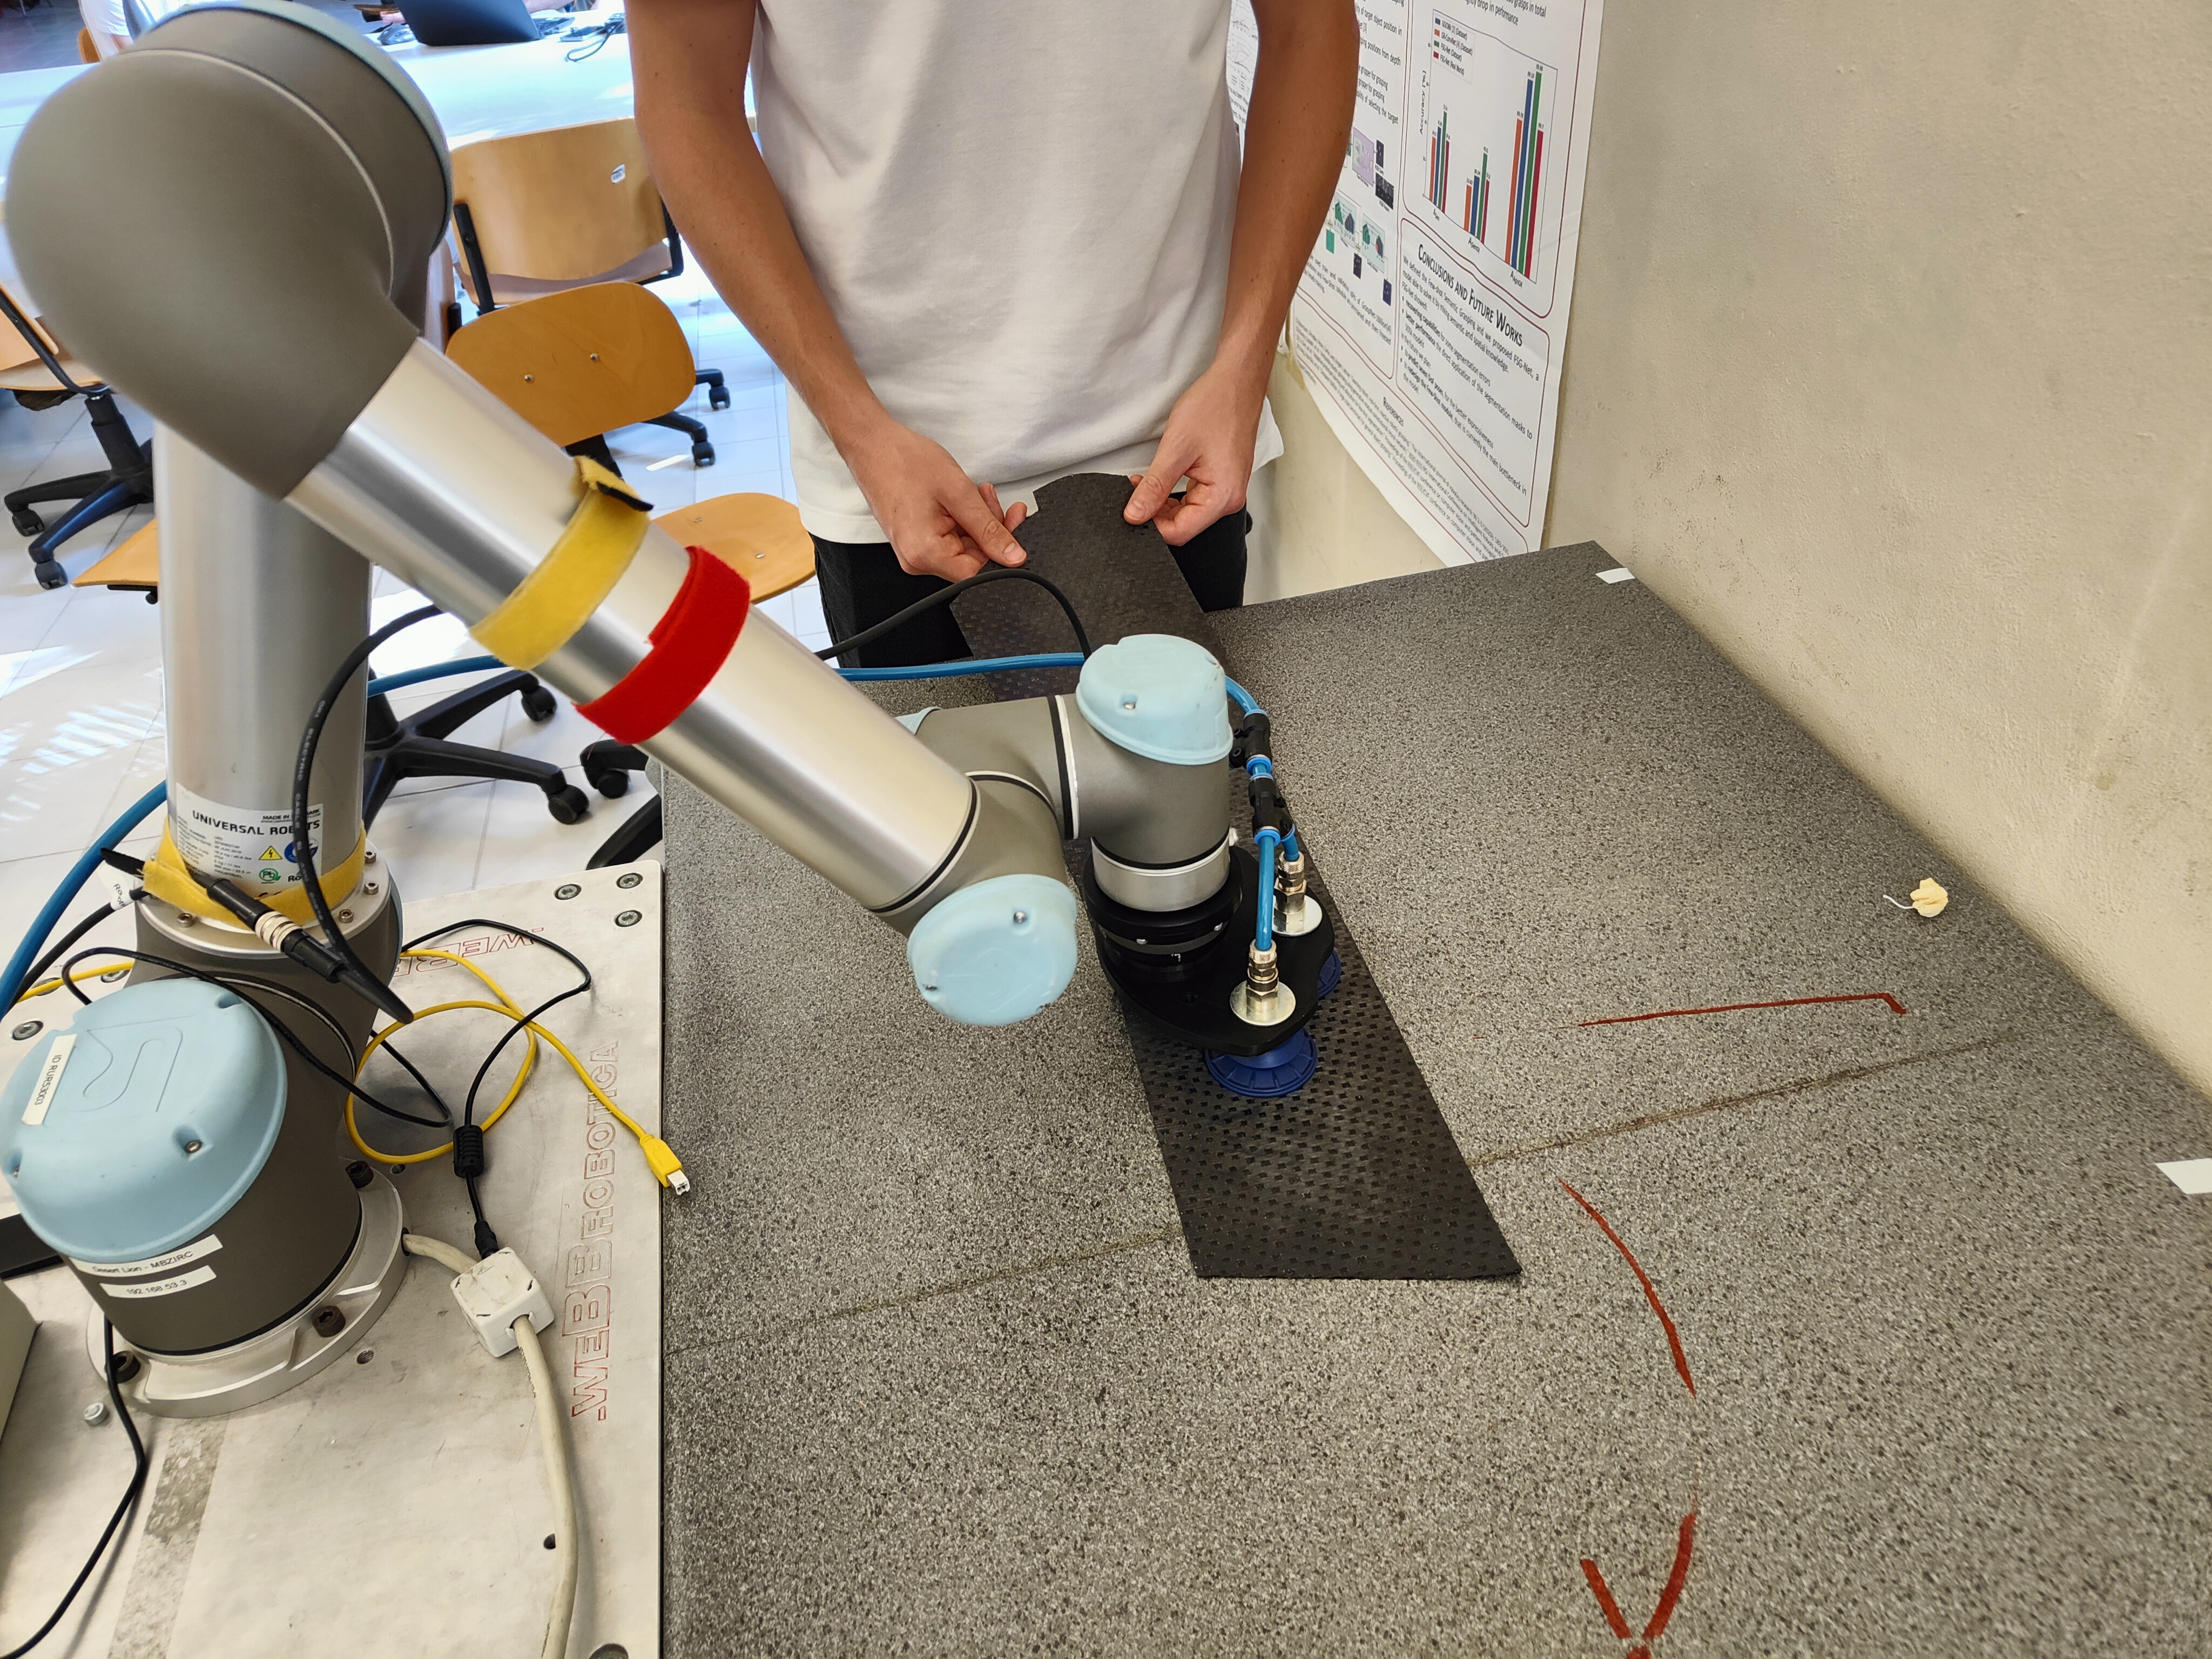
\includegraphics[width=\textwidth]{images/co-op1.jpg}
        \label{fig:co-op1}
    \end{subfigure}
    \qquad
    \begin{subfigure}[b]{0.45\textwidth}
        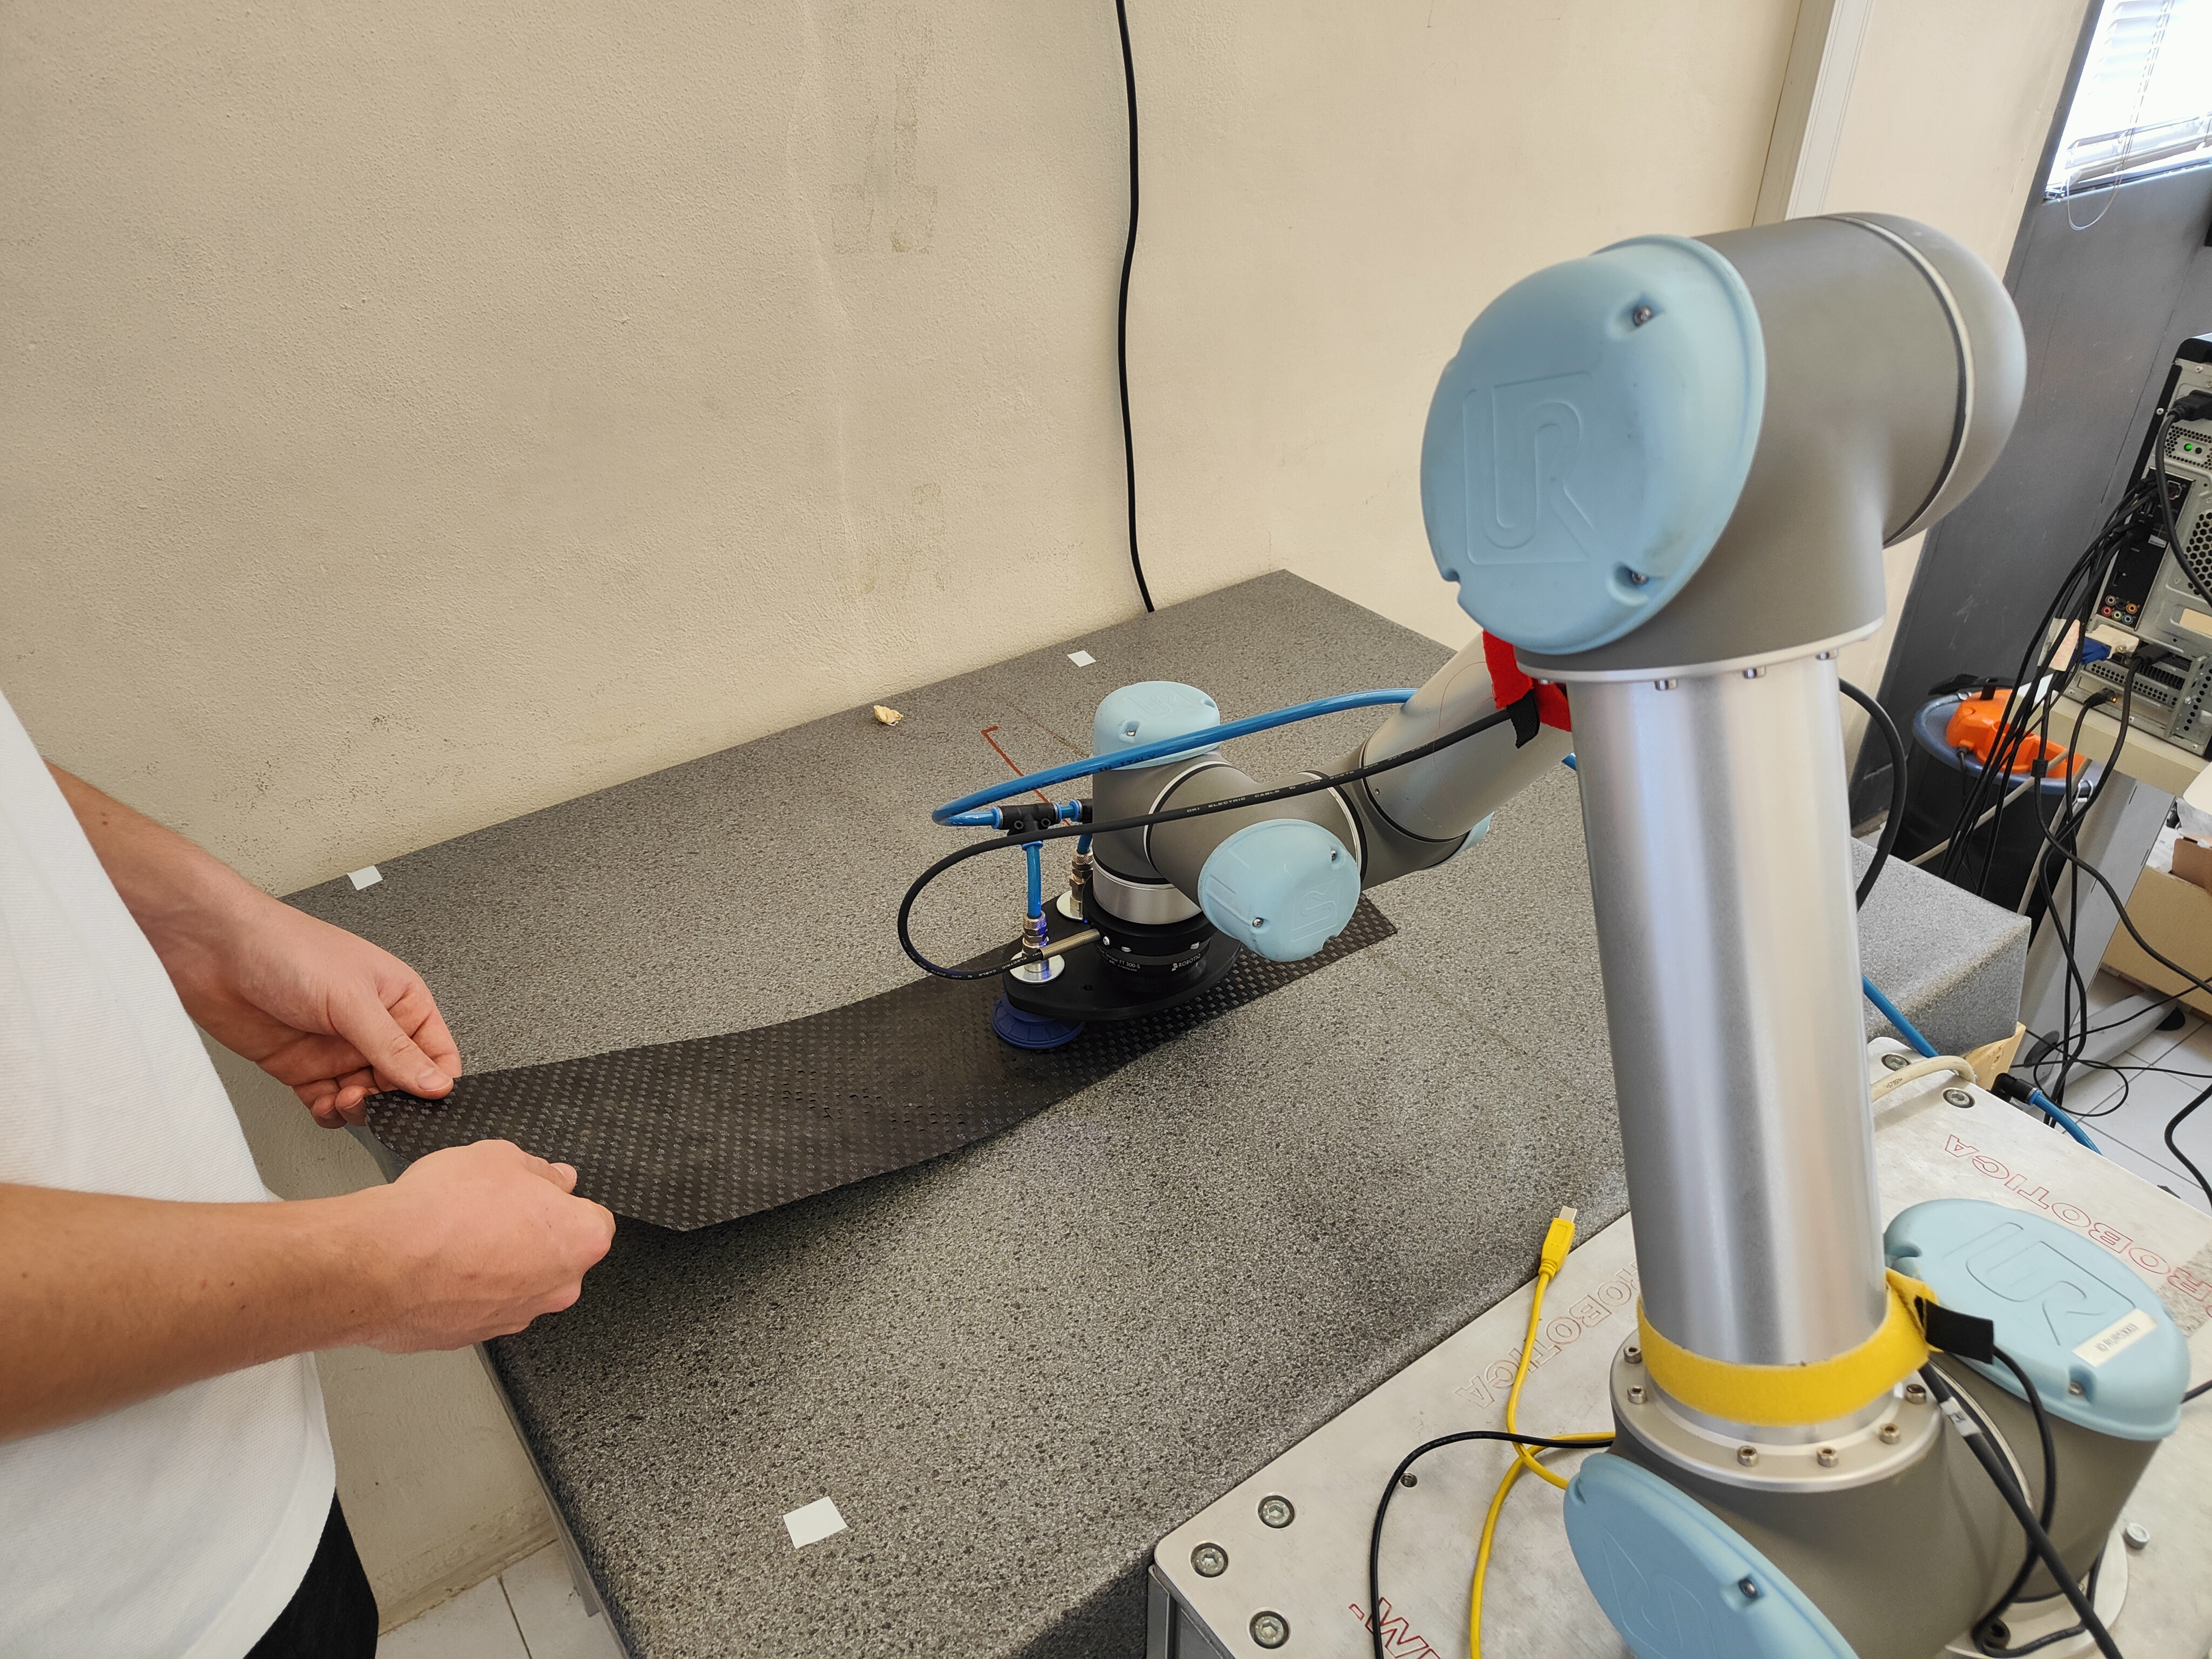
\includegraphics[width=\textwidth]{images/co-op2.jpg}
        \label{fig:co-op2}
    \end{subfigure}
    \caption{Applicazione di trasporto collaborativo, dove il robot segue i movimenti della persona in base alla lettura del sensore di forza}\label{fig:co-op}
\end{figure}
Con l'ausilio dell'\textit{inseguitore di forza}, si potr\'{a} poi trasportare e ruotare la lamina in collaborazione con il robot. 
\footnotetext{\url{https://github.com/andreastocco01/ur5_ft_tasks/blob/main/src/full_velocity_force_follower.cpp}}
 %File in cui verrà scritto il capitolo

\clearpage{\pagestyle{plain}\cleardoublepage} %Comando per iniziare il capitolo su pagina dispari
\chapter{Conclusioni} %Nome capitolo
\label{chapter:chapter6} %Label per creare riferimenti al capitolo
Gli esperimenti condotti in questa tesi hanno dimostrato che il sensore coppia-forza \'{e} uno strumento affidabile e preciso. 
Prima ne \'{e} stata valutata la reattivit\'{a} attraverso il cambiamento istantaneo delle forze applicate ad esso, 
successivamente ne \'{e} stata analizzata la precisione, utilizzando le piccole forze rilevate per calcolare la viscosit\'{a} del 
burro d'arachidi. 
In entrambi i casi, i risultati ottenuti sono ripetibili e coerenti con gli obiettivi specificati inizialmente. 
Sono state, poi, mostrate diverse applicazioni molto diffuse in letteratura come, ad esempio, il pick and place anche se, per 
quest'ultima, non sarebbe necessario disporre di un sensore coppia-forza. La tesi ha mostrato come l'interpretazione 
delle forze applicate al braccio possano incrementare la versatilit\'{a} e l'efficacia dell'applicazione nonch\'{e} l'esperienza 
utente. Utilizzando l'inseguitore di forza \'{e} possibile istruire il robot sulle posizioni variabili degli oggetti e, 
facendo una stima sull'altezza di essi, il braccio potr\'{a} effettuare una presa pi\'{u} solida e precisa. 
\'{E} stata presentata anche una variazione nel caso in cui non sia nota precisamente la posizione obiettivo. Utilizzando i dati 
del sensore si riesce a dedurre se ci si trova o meno al di sopra della cavit\'{a} in cui inserire l'oggetto. 
\'{E} stato, inoltre, presentato un esempio di trasporto collaborativo, con il quale il robot aiuta l'operatore nel trasporto 
di un materiale sottile e leggero. 
La tesi ha delineato alcune possibili direzioni per migliorare ulteriormente le prestazioni delle applicazioni presentate. 
Ci\'{o} include, ad esempio, l'integrazione di telecamere e l'intelligenza artificiale per migliorare ulteriormente la capacit\'{a} 
di percezione e controllo del robot. 
In conclusione, la tesi ha confermato l'importanza e l'utilità del sensore coppia-forza nelle applicazioni robotiche, 
offrendo spunti per il suo miglioramento e indicando possibili sviluppi futuri. L'utilizzo dei sensori coppia-forza apre 
nuove possibilità nel controllo e nella manipolazione degli oggetti, contribuendo alla crescita e all'evoluzione 
della robotica industriale. %File in cui verrà scritto il capitolo

\clearpage{\pagestyle{plain}\cleardoublepage}
\nocite{yt_tutorial}
\nocite{moveit_tutorial}
\nocite{cao2021six}
\nocite{lee2015capacitive}
\nocite{ur5}
\printbibliography[nottype=online, heading=subbibliography, title=Bibliografia, heading=bibintoc]
\clearpage{\pagestyle{plain}\cleardoublepage}
\printbibliography[type=online, heading=subbibliography, title=Sitografia, heading=bibintoc]
\end{document}